
The layout component is responsible for finding a mapping to storage that takes into account information that are available through the conceptional and logical views to the data.
In addition, this section addresses some aspects that explain how the mapping is driven by performance models and the site configuration.


%%%%%%%%%%%%%%%%%%%%%%%%%%%%%%%%%%%%%%%%%%%%%%
\subsection{Logical View}

\begin{figure}
	\centering
	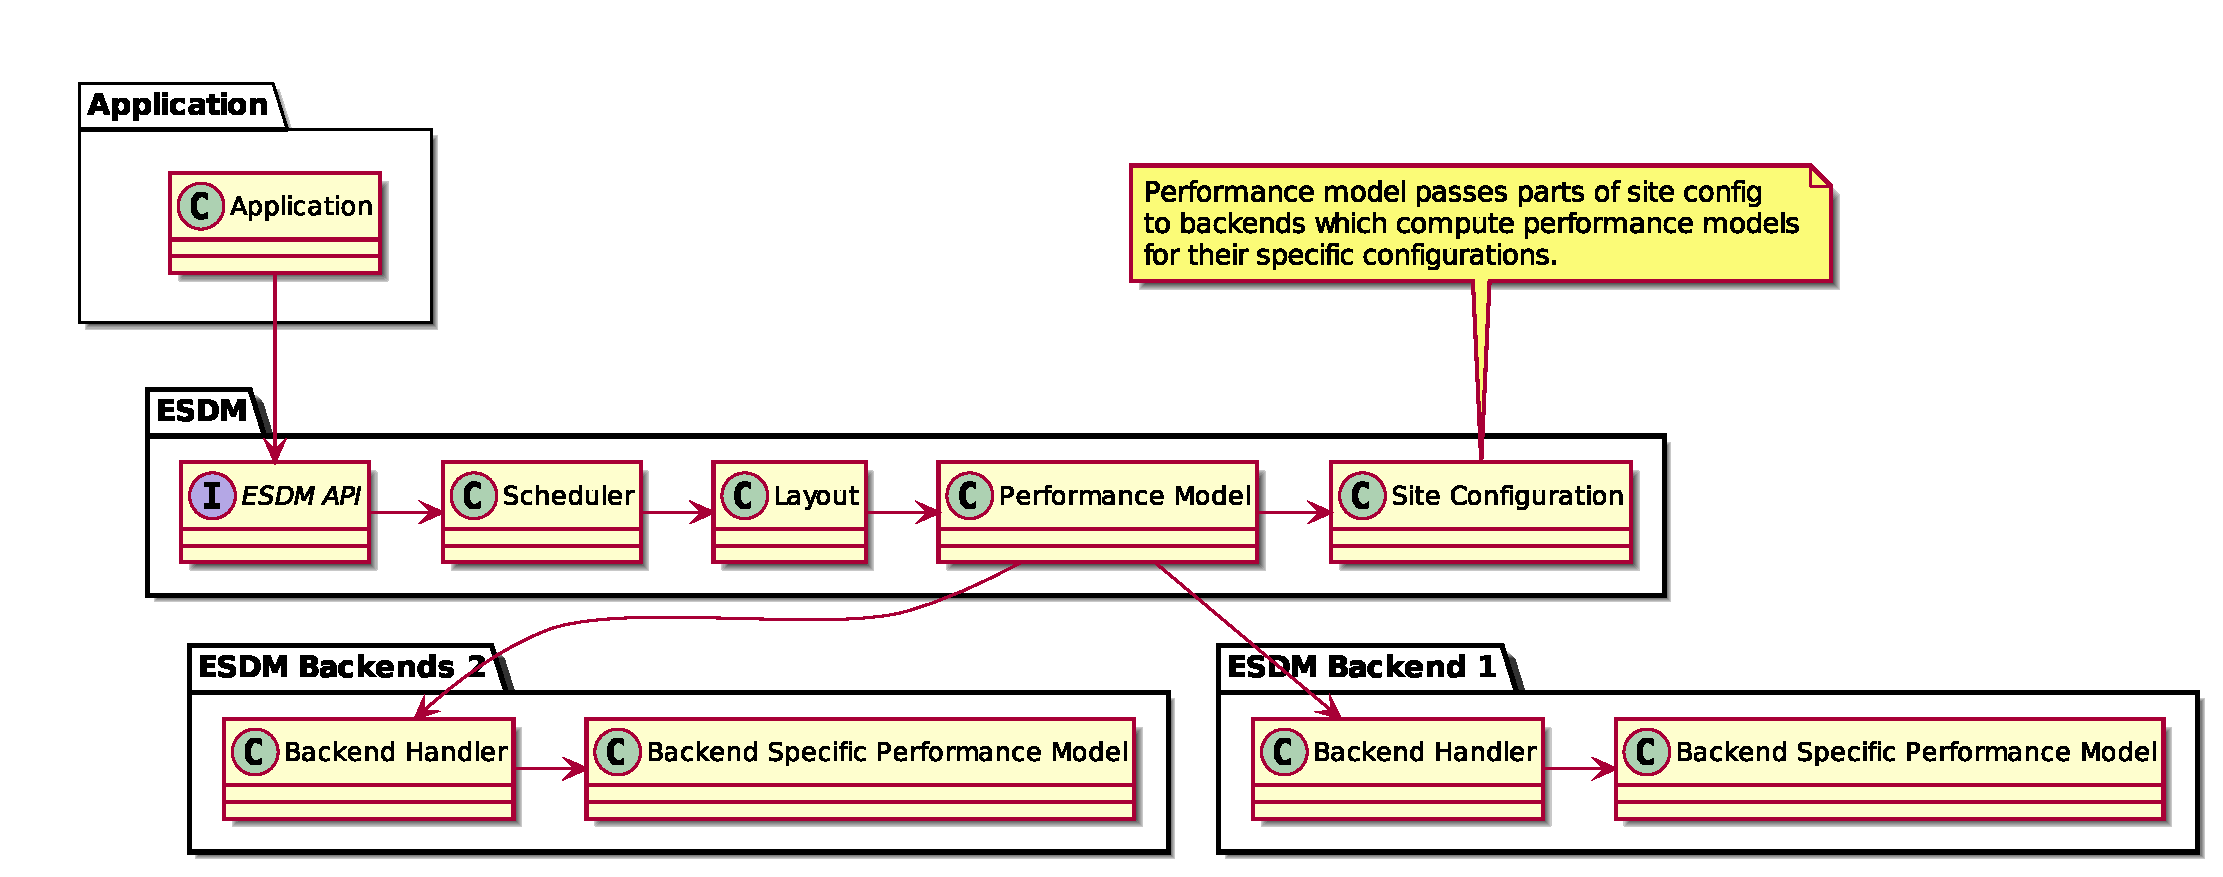
\includegraphics[width=\linewidth]{esdm-components/layout/logical.eps}
	\caption{An application that is using ESDM interfaces through the ESDM API (which in many cases maybe only read/write calls). Eventually the scheduling component has to consult the layout component which is responsible for returning a list of Fragments which have to be read or written. To provide this list the performance model is used which in turn queries the available backends and the site configuration for an estimate.}
	\label{fig:esdm layout logical view}
\end{figure}

The layout component is invoked by the ESDM scheduler to break down incoming requests into fragments that are beneficial from a data access and storage perspective.
The layout components responsibilities in more detail include the following:

\begin{itemize}
	\item map (e.g., a domain) to fragments
	\item where to save new/additional/replica fragments?
	\item time estimates for reading a fragment (e.g., a callback per backend and configuration provided)
	\item time estimates for writing a fragment, in particular find a domain mapping
\end{itemize}

\Cref{fig:esdm layout logical view} illustrates the embedding of the layout component into the larger ESDM architecture.
To find a mapping an important factor is the performance of the individual backends, which requires to know which backends are available.
\Cref{sec:layout/logical/init} describes the initialisation process that loads the site configuration.
Storage backends feature wildly different performance characteristics, which is why the ESDM features an abstract performance model that queries the individual ESDM backends to provide performance estimates which may also depend on the data structure of the request.
\Cref{sec: layout/logical/decision} describes the performance model and decision process in more detail.

\subsubsection{Initialisation of the Layout/Performance Model}
\label{sec:layout/logical/init}

The layout decision requires knowledge of the available backends.
The ESDM assumes a machine-friendly site configuration to be available.
The site configuration includes a list of available backends for which the ESDM on initialisation loads.
\Cref{fig:esdm layout initialisation} shows a UML sequence diagram of the ESDM initialisation process.

\begin{enumerate}
	\item Application/Library: calls ESDM initialisation
	\item ESDM:
	\begin{enumerate}
		\item reads configuration file
		\item discovers and loads available backends + plugins + backend performance model
		\item available backends are announced to the ESDM performance model for consideration
	\end{enumerate}
	\item After successful initialisation control is returned to the calling application/library.
\end{enumerate}

\begin{figure}
	\centering
	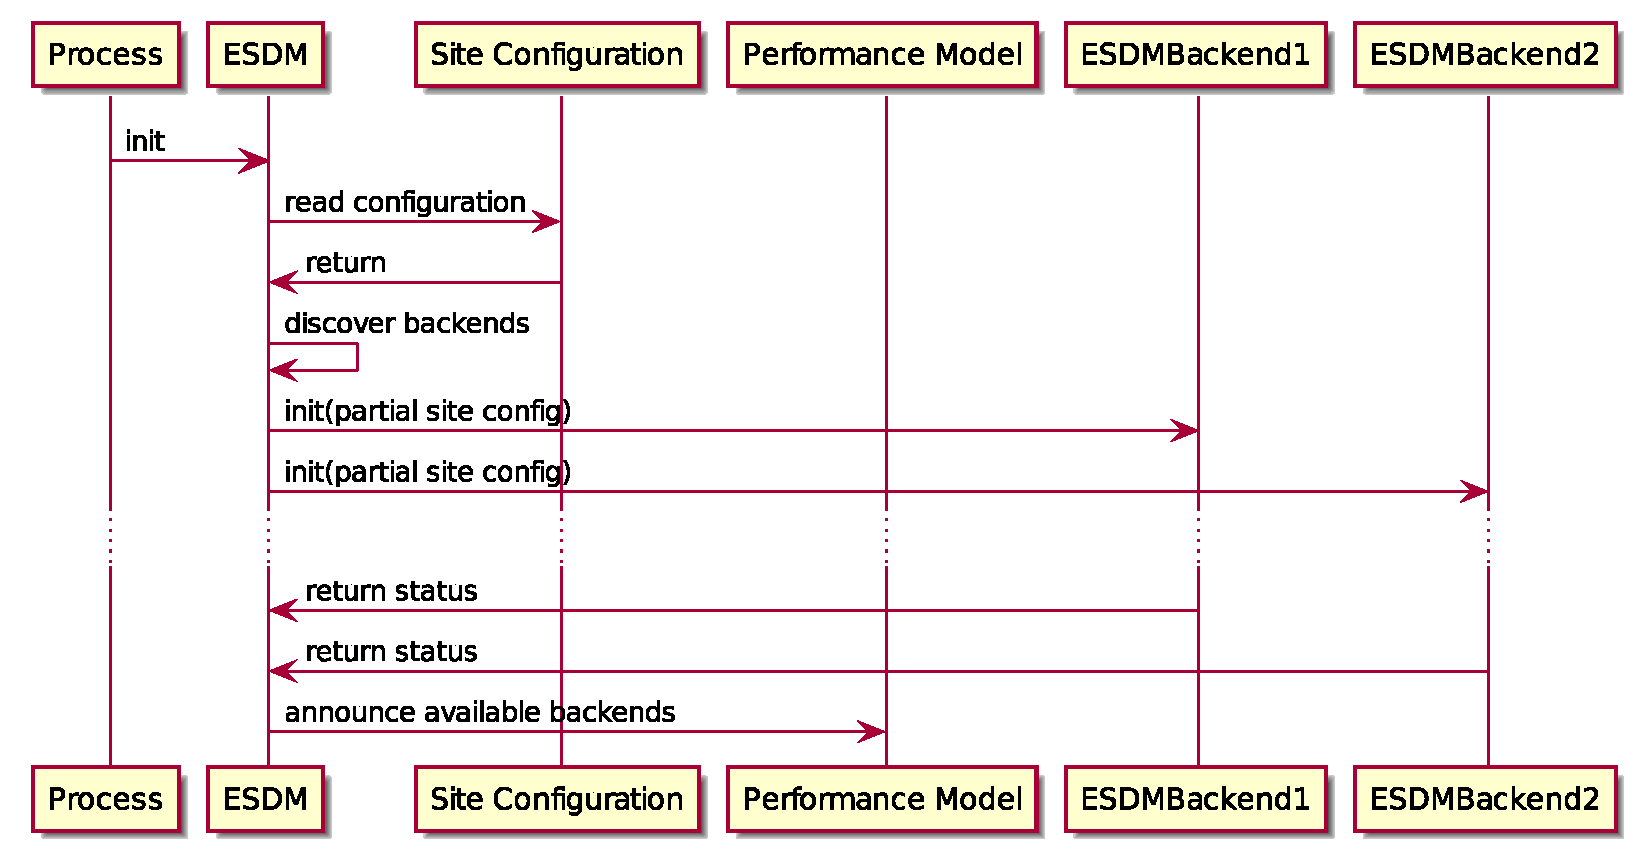
\includegraphics[width=\linewidth]{esdm-components/layout/sequence_init.eps}
	\caption{The initialisation process of the ESDM and the performance model and also the available backends.}
	\label{fig:esdm layout initialisation}
\end{figure}



\subsubsection{Performance Model and Decision Process}
\label{sec: layout/logical/decision}

One approach to find the best backend/backends is to query every backend for a performance estimate and choose the most affordable.
\Cref{fig:esdm layout choose backend} shows in a simplified example how the decision process for a data centre with three storage systems may look like.
The decision would gather estimates by calling the performance model (PM) of every backend.
Performance metrics may include:

\begin{itemize}
	\item Latency
	\item Throughput (read/write)
	\item Energy/Cost
	\item Capacity/Fill level
\end{itemize}

Users or administrators may weight which factors are most important for their application.
The decision process has to be configurable because different sites have different requirements.

\begin{figure}
	\centering
	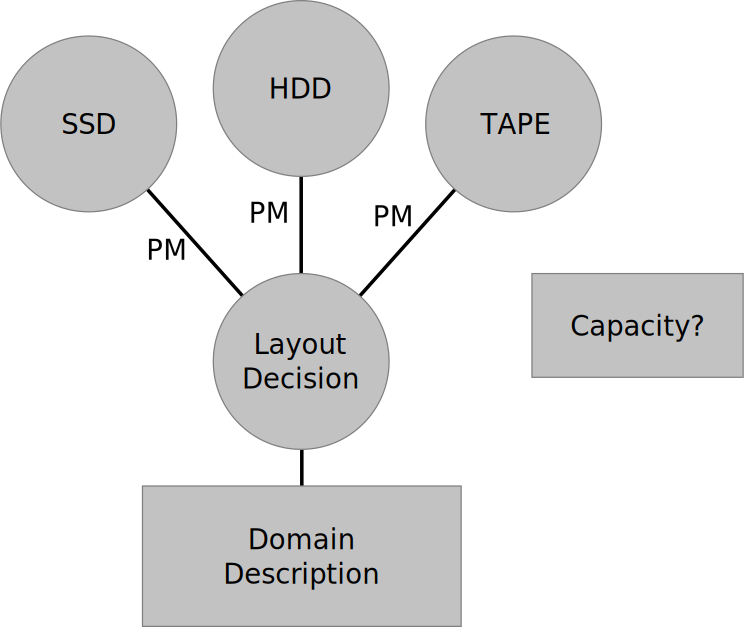
\includegraphics[width=0.5\linewidth]{esdm-components/layout/performance-model.pdf}
	\caption{A layout decision component queries the performance estimates for every backend and also takes the domain into account. Possibly other metrics such as the available capacity for every backend may as well be considered.}
	\label{fig:esdm layout choose backend}
\end{figure}

% Unadressed: When to release allocated memory?


\subsubsection{Layout Reconstruction}

When applications are reading data the ESDM Scheduler consults the layout component for a domain reconstruction.
A subdomain description is passed to the layout component as part of request.
The layout component then requests metadata for the container/variable to be received.
From the list of available fragments the layout component has now to choose a subset of fragments that can be read efficiently from the backends.
To decide which fragments to choose the performance model is consulted.


%%%%%%%%%%%%%%%%%%%%%%%%%%%%%%%%%%%%%%%%%%%%%%
\subsection{Process View}

For the layout component to types of processes can be distinguished:

\begin{itemize}
	\item Layout reconstructions and finding fragmentation
	\item Gathering performance estimates
\end{itemize}

\Cref{fig:esdm layout process view} illustrates the possible process in am UML diagram.
Layout reconstructions may result in multiple requests to multiple ESDM backends.
How ESDM gathers/flushes these fragments concurrently is described in \Cref{component: scheduler}.


\begin{figure}
	\centering
	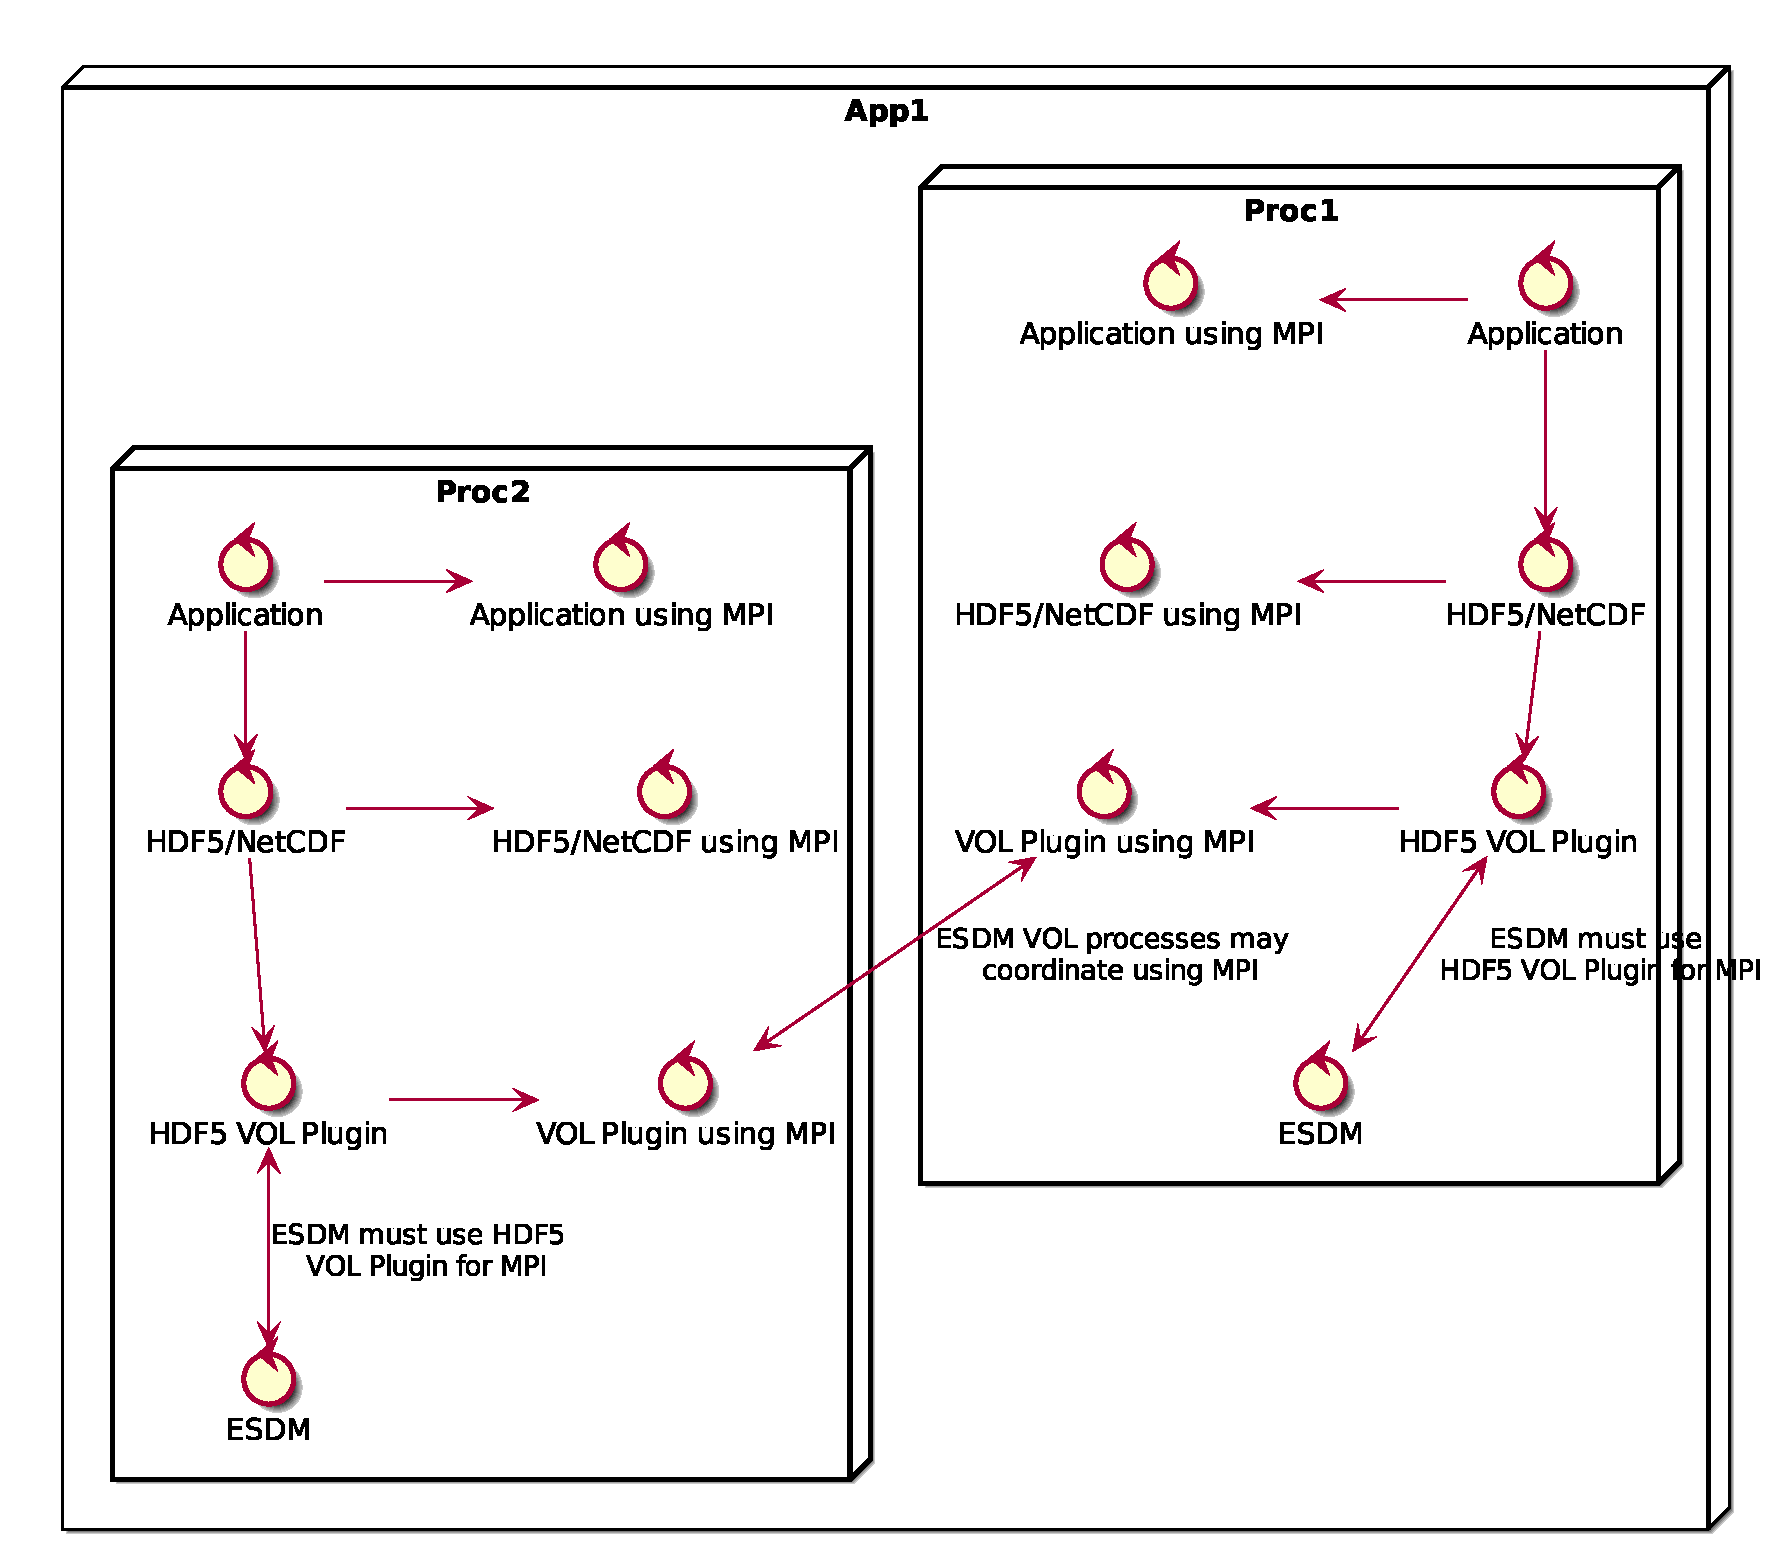
\includegraphics[width=\linewidth]{esdm-components/layout/process.eps}
	\caption{Multiple process are involved with most applications. For every node the performance decisions maybe different, but in many cases it also maybe desirable to find an estimate collectively. Ultimately the performance estimate needs to be relatively cheap to compute. }
	\label{fig:esdm layout process view}
\end{figure}





%%%%%%%%%%%%%%%%%%%%%%%%%%%%%%%%%%%%%%%%%%%%%%
\subsection{Physical View}

\begin{figure}
	\centering
	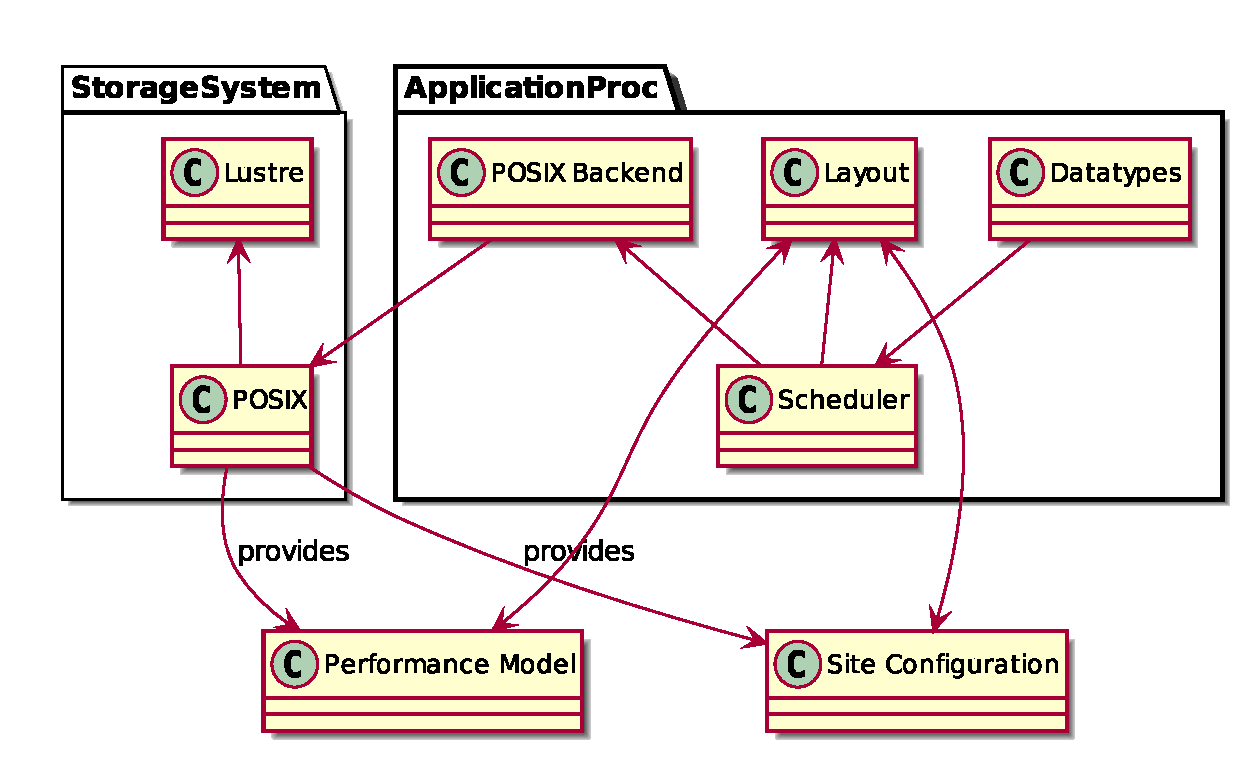
\includegraphics[width=\linewidth]{esdm-components/layout/physical.eps}
	\caption{Physical view for the layout component a closely related components.}
	\label{fig:esdm layout  physical view}
\end{figure}

The layout component relies on multiple subcomponents, all of which only exist within the application process.
\Cref{fig:esdm layout physical view} illustrates the distribution and relation of the components across different hardware components.
The site configuration is expected to be pulled from a storage system that can withstand a large number of reading clients.
Nodes may cache the site configuration locally.
The ESDM layout component does require prerequisites from the storage system, but changes to the configuration of the storage system should be reflected in the site configuration.


%%%%%%%%%%%%%%%%%%%%%%%%%%%%%%%%%%%%%%%%%%%%%%%
%\subsection{Development View}
%
%\begin{figure}
%	\centering
%	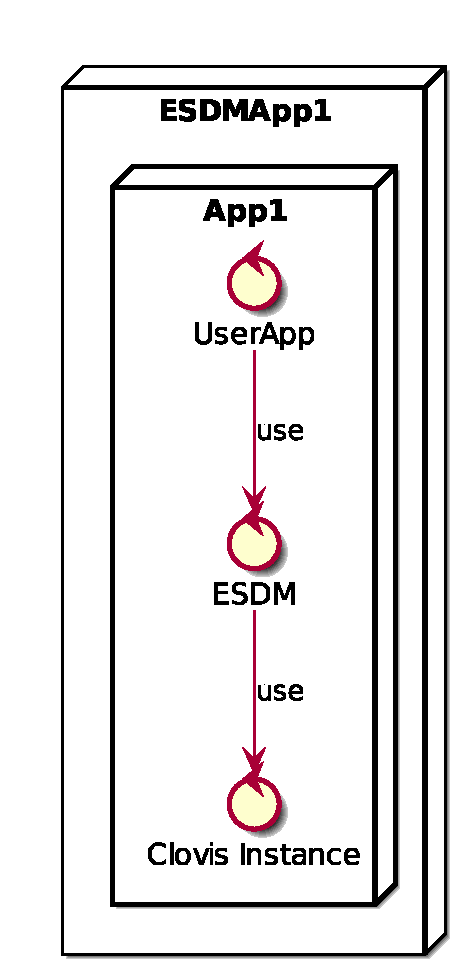
\includegraphics[width=\linewidth]{esdm-layout/development.eps}
%	\caption{}
%	\label{fig:esdm layout development view}
%\end{figure}
